\newcommand{\sumi}{\sum\limits_{n=0}^\infty}

\section{Лекция номер 9}
\begin{conj}
    Есть функция $f: E \subset \C \longrightarrow \C$, а также точка $z_0 \in \Int E$. Функция $f$ дифференцируема в точке $z_0$, если $\exists k \in \C$, такое, что: 
    \begin{gather*}
        f(z) = f(z_0) + k(z - z_0) + o(z - z_0) \text{ при } z \longrightarrow z_0
    \end{gather*}
    $k$ -- производная $f$ в точке $z_0$
\end{conj}
\notice
\begin{enumerate}
    \item $k$ считается как:
    \begin{gather*}
        k = \lim\limits_{z \longrightarrow z_0} \frac{f(z) - f(z_0)}{z - z_0}
    \end{gather*}
    \item Существование производной равносильно дифференцируемости.
\end{enumerate}
\begin{theorem}
    Пусть $R$ -- радиус сходимости ряда $\sumi a_n(z - z_0)^n$, тогда $f(z) = \sumi a_n(z-z_0)$
    бесконечно дифференцируема в круге $\abs{z - z_0} < R$ и ее производную мы можем посчитать следующим образом:
    \begin{gather*}
        f^{(m)} = \sum\limits_{n=m}^\infty n(n-1)\dots (n-m+1)a_n(z-z_0)^{n-m} 
    \end{gather*}
\end{theorem}
\begin{proof}
    Для простоты формул зафиксируем $z_0 = 0$. Возьмем некое $r \in (0, R)$ и две точки, лежащие в маленьком круге: $\abs{z}, \abs{w} < r$. Тогда:
    \begin{gather*}
        \frac{f(w) - f(z)}{w - z} = \sum\limits_{n=0}^\infty a_n \cdot \frac{w^n - z^n}{w - z} = \sum\limits_{n=1}^\infty a_n (w^{n-1} + w^{n-2} z + \dots + z^{n-1}) 
    \end{gather*} 
    Пририсуем предел с обеих сторон:
    \begin{gather*}
        f'(z) = \lim\limits_{w \rightarrow z} \frac{f(w) - f(z)}{w - z} = \lim\limits_{w \rightarrow z} \sum\limits_{n=1}^\infty a_n (w^{n-1} + w^{n-2} z + \dots + z^{n-1}) = \oast 
    \end{gather*}
    Хотим переставить местами сумму с пределом, мы можем это сделать, когда ряд равномерно сходится. $z$ фиксировано, значит хотим проверить равномерную сходимость по $w$. Чтобы 
    проверить равномерную сходимость промажорируем ряд и применим Вейерштрасса:
    \begin{gather*}
        \abs{a_n (w^{n-1} + w^{n-2} z + \dots + z^{n-1})}  \leqslant \abs{a_n} (\abs{w}^{n-1} + \abs{w}^{n-2} \abs{z} + \dots + \abs{z}^{n-1}) \leqslant \abs{a_n} \cdot n r^{n-1}
    \end{gather*}
    Мы выясняли, что радиус сходимости у $\sum a_n z^n$ равен радиусу сходимости $\sum n a_n z^{n-1}$ сходится. 
    Значит радиус сходимости $\sum n a_n z^{n-1}$ равен $R$. Значит в любой точке $R$ он абсолютно сходится. 
    При этом $r$ у нас из круга, так что $\sum \abs{a_n} \cdot n r^{n-1}$ будет сходится. Значит мы промажорировали наш ряд чем-то, что не зависит от $w$ и сходится. 
    Получаем необходимую равномерную сходимость и меняем местами сумму с пределом:
    \begin{gather*}
        \oast = \sum\limits_{n=1}^\infty \lim\limits_{w \rightarrow z} a_n (w^{n-1} + w^{n-2} z + \dots + z^{n-1}) = \sum\limits_{n=0}^\infty n a_n z^{n-1}
    \end{gather*}
    Нучились дифференцировать один раз, дальше доказываем формулу по индукции. Радиус сходимости не изменился, значит все хорошо. 
\end{proof}
\begin{theorem}
    (Единственность разложени функции степенной ряд)
    
    Пусть есть функция, разложенная в степенной ряд:
    \begin{gather*}
        f(z) = \sumi a_n (z - z_0)^n \text{ при } \abs{z - z_0} < R
    \end{gather*}
    Тогда:
    \begin{gather*}
        a_n = \frac{f^{(n)}(z_0)}{n!}
    \end{gather*}
\end{theorem}
\begin{proof}
    По только что доказанной теореме: 
    \begin{gather*}
        f^{(m)}(z) = \sum\limits_{n=m}^\infty n(n-1)\dots (n-m+1)a_n (z-z_0)^{n-m}
    \end{gather*}
    Если посмотреть на $f^{(m)}(z_0)$, то мы видим, 
    что все всегда зануляется из за последнего множетеля. За исключением случая $m=n$. Тогда мы получаем: 
    \begin{gather*}
        f^{(m)}(z_0) = n(n-1) \dots 1 \cdot a_n = a_n \cdot n!
    \end{gather*}
    Получили нужную формулу для коэффициентов. Единственность следует из единственности проивзодной.
\end{proof}
\begin{conj}
    Ряд Тейлора для функции $f$ в точке $z_0$:
    \begin{gather*}
        \sumi \frac{f^{(n)}(z_0)}{n!} (z - z_0)^n
    \end{gather*}
\end{conj}
\begin{conj}
    Функция называется \textbf{аналитической} в точке $z_0$, если она бесконечно 
    дифференцируема и является суммой своего ряда Тейлора в некой окрестности $z_0$:
    \begin{gather*}
       f(z) = \sumi \frac{f^{(n)}(z_0)}{n!} (z - z_0)^n 
    \end{gather*}
\end{conj}
\notice \; Просто бесконечной дифференцируемости функции в общем случае недостаточно для аналитичности.

\textbf{Пример:} 
\begin{gather*}
    f(x) = \begin{cases}
        e^{-1/x^2} \text{ при } x \neq 0 \\
        0 \text{ при } x = 0
    \end{cases} 
\end{gather*} 
Утверждаем, что она бесконечно дифференцируема, но не раскладывается в свой ряд Тейлора в нуле. 
\begin{proof}
    Для начала посмотрим на производные в точках, отличных от нуля.
    По индукции докажем, что при $x \neq 0$:
    \begin{gather*}
        f^{(n)}(x) = \frac{P_n(x)}{x^{3n}} \cdot e^{-1/x^2}
    \end{gather*}
    Где $P_n(x)$ -- некий многочлен. База очевидна, дробь слева равна 1. Переход $n \longrightarrow n + 1$:
    \begin{gather*}
        f^{(n+1)}(x) = \left( \frac{P_{n}(x)}{x^{3n}} e^{-1/x^2} \right)' = \left( P_{n}(x)x^{-3n} e^{-1/x^2} \right)' = \\
        P_{n}'(x)x^{-3n} e^{-1/x^2} + P_{n}(x)(-3n x^{-3n-1}) e^{-1/x^2} + P_{n}(x)x^{-3n} e^{-1/x^2} \cdot \frac{2}{x^3} = \\ 
        \frac{e^{-1/x^2}}{x^{3n+3}}(x^3 P_n'(x) - 3nx \cdot P_n(x) + P_n(x))
    \end{gather*}
    Теперь дифференцируем в нуле. Докажем по индукции, что $f^{(n)}(0) = 0$. База очевидна из условия. Переход $n \longrightarrow n+1$:
    \begin{gather*}
        f^{(n+1)}(0) = \lim\limits_{x \rightarrow 0} \frac{f^{(n)}(x) - \stackabove{f^{(n)}(0)}{0}}{x} = \lim\limits_{x \rightarrow 0} \frac{P_n(x)e^{-1/x^2}}{x^{3n+1}} = 
        \lim\limits_{x \rightarrow 0} P_n(x) \cdot \underbrace{\colorboxed{red}{\frac{e^{-1/x^2}}{x^{3n+1}}}}_{\rightarrow 0} = 0
    \end{gather*}
    Что мы получили? Мы получили дифференцируемость во всех точках.
    Теперь попробуем разложить $f$ в ряд Тейлора в нуле. Это какая-то хрень из нулей потому что в нуле все производные ноль:
    \begin{gather*}
        \sumi 0 \cdot x^n \equiv 0 
    \end{gather*}
    Это очевидно неверно, значит $f$ не является суммой своего ряда Тейлора, а значит она не аналитична. 
\end{proof}
% Знаешь что, Линский? Я в своем познании настолько преисполнился, что я как будто бы уже
% сто триллионов миллиардов лет проживаю на триллионах и
% триллионах таких же планет, как эта Земля, мне этот мир абсолютно
% понятен, и я здесь ищу только одного - покоя, умиротворения и
% вот этой гармонии, от слияния с бесконечно вечным, от созерцания
% великого фрактального подобия и от вот этого замечательного всеединства
% существа, бесконечно вечного, куда ни посмотри, хоть вглубь - бесконечно
% малое, хоть ввысь - бесконечное большое, понимаешь? А ты, Линский мне опять со
% своим вот этим, иди суетись дальше, это твоё распределение, это
% твой путь и твой горизонт познания и ощущения твоей природы, он
% несоизмеримо мелок по сравнению с моим, понимаешь? Я как будто бы уже
% давно глубокий старец, бессмертный, ну или там уже почти бессмертный,
% который на этой планете от её самого зарождения, ещё когда только Солнце
% только-только сформировалось как звезда, и вот это газопылевое облако,
% вот, после взрыва, Солнца, когда оно вспыхнуло, как звезда, начало
% формировать вот эти коацерваты, планеты, понимаешь, я на этой Земле уже
% как будто почти пять миллиардов лет живу и знаю её вдоль и поперёк
% этот весь мир, а ты, Линский мне какие-то... мне не важно на твои тачки, на твои
% яхты, на твои квартиры, там, на твоё благо. Я был на этой
% планете бесконечным множеством, и круче Цезаря, и круче Гитлера, и круче
% всех великих, понимаешь, был, а где-то был конченым говном, ещё хуже,
% чем здесь. Я множество этих состояний чувствую. Где-то я был больше
% подобен растению, где-то я больше был подобен птице, там, червю, где-то
% был просто сгусток камня, это всё есть душа, понимаешь? Она имеет грани
% подобия совершенно многообразные, бесконечное множество. Но тебе этого
% не понять, поэтому ты, Линский езжай себе , мы в этом мире как бы живем
% разными ощущениями и разными стремлениями, соответственно, разное наше и
% место, разное и наше распределение. Тебе я желаю все самые крутые тачки
% чтоб были у тебя, и все самые лучше самки, если мало идей, обращайся ко 
% мне, я тебе на каждую твою идею предложу сотню триллионов, как всё делать. 
% Ну а я всё, я иду как глубокий старец,узревший вечное, прикоснувшийся к Божественному, 
% сам стал богоподобен и устремлен в это бесконечное, и который в умиротворении, покое, гармонии, благодати, 
% в этом сокровенном блаженстве пребывает, вовлеченный во всё и во вся, понимаешь, вот и всё, в этом наша разница. 
% Так что я иду любоваться мирозданием, а ты, Линский идёшь преисполняться в ГРАНЯХ каких-то, вот и вся разница, понимаешь, 
% ты, Линский не зришь это вечное бесконечное, оно тебе не нужно. Ну зато ты, Линский, так сказать, более активен, как вот этот дятел долбящий, 
% или муравей, который очень активен в своей стезе, поэтому давай, наши пути здесь, конечно, имеют грани подобия, потому 
% что всё едино, но я-то тебя прекрасно понимаю, а вот ты, Линский меня - вряд ли, потому что я как бы тебя в себе содержу, 
% всю твою природу, она составляет одну маленькую там песчиночку, от того что есть во мне, вот и всё, поэтому давай, 
% ступай, езжай, а я пошел наслаждаться прекрасным осенним закатом на берегу теплой южной реки. Всё, ступай, и я пойду.
\vspace*{5mm}
\underline{Разложение элементарных функций в ряд Тейлора:}

\begin{align*}
    1. \; e^x &= \sumi \frac{x^n}{n!} & 2. \; \cos{x} &= \sumi \frac{(-1)^n x^{2n}}{(2n)!} & 3. \; \sin{x} = \sumi \frac{(-1)^n x^{2n+1}}{(2n+1)!}
\end{align*}
Эти ряды сходятся во всей плоскости, так что мы также можем определить $e^z, \cos{z}$ и $\sin{z}$ для $z \in \C$.
И тогда станет понятно, откуда растут ноги у формулы Эйлера:
\begin{gather*}
    e^{iz} = \cos{z} + i\sin{z}
\end{gather*}
Отсюда же берется и следующий набор формул:
\begin{align*}
    1. \; e^{z+w} &= e^z \cdot e^w & 2. \; \sin^2{z} + \cos^2{z} &= 1 & 3. \; \sin{z} &= \frac{e^{iz} - e^{-iz}}{2i} & 4. \; \cos{z} &= \frac{e^{iz} + e^{-iz}}{2}
\end{align*}
Заведем еще одно разложение:
\begin{gather*}
    4. \; \ln(1+x) = \sum\limits_{n=1}^\infty \frac{(-1)^{n-1}x^n}{n} \text{ при } x \in (-1, 1)
\end{gather*}
\begin{proof}
    Начнем с того, что:
    \begin{gather*}
        \frac{1}{1 + t} = \sumi (-1)^n t^n \text{ сходится при } \abs{t} < 1
    \end{gather*}
    Тогда можем проинтегрировать такую штуку в круге сходимости:
    \begin{gather*}
        \ln(1 + x) = \int\limits_0^x \frac{dt}{1+t} = \int\limits_0^x \sumi (-1)^n t^n dt = \sumi \int\limits_0^x (-1)^n t^n dt = 
        \sum\limits_{n=0}^\infty \frac{(-1)^{n}x^{n+1}}{n+1}
    \end{gather*}
\end{proof}
Разложим что нибудь еще, нам же абсолютно нечем заняться:
\begin{gather*}
    5. \; \arctg{x} = \sumi \frac{(-1)^n x^{2n+1}}{2n+1} \text{ при } x \in (-1, 1]
\end{gather*}
В частности:
\begin{gather*}
    \frac{\pi}{4} = 1 - \frac{1}{3} + \frac{1}{5} - \frac{1}{7} + \frac{1}{9} - \dots 
\end{gather*}
\begin{proof}
    \begin{gather*}
        \frac{1}{1+t^2} = \sumi (-1)^n t^{2n} \text{ сходится при } \abs{t} < 1 \\
        \arctg{x} = \int\limits_{0}^x \frac{dt}{1+t^2} = \sumi \int\limits_{0}^x (-1)^n t^{2n} dt = \sumi \frac{(-1)^n x^{2n+1}}{2n+1}
    \end{gather*}
    Теорема Абеля: Если ряд сходится в 1, то его сумма $ = \lim\limits_{x \rightarrow 1-} \sum a_n x^n$. Тогда:
    \begin{gather*}
        \sumi \frac{(-1)^n}{2n+1} = \lim\limits_{x \rightarrow 1-} \sumi \frac{(-1)^n x^{2n+1}}{2n+1} = \lim\limits_{x \rightarrow 1-} \arctg{x} = \arctg{1} = \frac{\pi}{4}
    \end{gather*}
\end{proof}
И снова на те же грабли:
\begin{gather*}
    6. \; (1+x)^p = 1 + \sum\limits_{n=1}^\infty \frac{p(p-1)\dots(p-n+1)}{n!}x^n \text{ при } x \in (-1, 1)
\end{gather*}
\begin{proof}
    Хотим доказать, что остаток стремится к нулю. Запишем его в интегральной форме:
    \begin{gather*}
        R_n(x) = \frac{1}{n!} \int\limits_0^x (x - t)^n (1+t)^{p-n+1} p(p-1)\dots(p-n+1)dt
    \end{gather*}
    Чтобы доказать, что он стремится к нулю, посмотрим на отношение соседних членов:
    \begin{gather*}
        \abs{\frac{R_{n+1}(x)}{R_n(x)}} = \frac{\abs{p-n}}{n+1} \cdot \frac{\abs{\int\limits_0^x (x - t)^{n+1}(1+t)^{p-n} dt}}{\abs{\int\limits_0^x (x - t)^{n}(1+t)^{p-n+1} dt}} = 
        \frac{\abs{p-n}}{n+1} \cdot \frac{\abs{\int\limits_0^x f(t) \frac{x-t}{1+t} dt}}{\abs{\int\limits_0^x f(t) dt}} = \oast 
    \end{gather*}
    Если взять $x =: -y, t =: -u$. То очевидно, что:
    \begin{gather*}
        \abs{\frac{-y + u}{1 - u}} = \frac{y - u}{1 - u} \leqslant y \Longrightarrow \abs{\frac{x - t}{1 + t}} \leqslant \abs{x}
    \end{gather*}
    Если приглядеться, то оба интеграла знакопостоянны, так что мы можем занести модуль под интеграл:
    \begin{gather*}
        \oast = \frac{\abs{p-n}}{n+1} \cdot \frac{\int\limits_0^x \abs{f(t)} \lessabove{\abs{\frac{x-t}{1+t}}}{\abs{x}} dt}{\int\limits_0^x \abs{f(t)} dt} \leqslant \bigstar  
    \end{gather*}
    Ну выходит эти интегралы у нас различаются не больше чем на $\abs{x}$, а $x < 1$, значит:
    \begin{gather*}
        \bigstar \leqslant \frac{\abs{p - n}}{n + 1} \cdot \abs{x} \leqslant (1+\varepsilon)\abs{x} \text{ при больших } n 
    \end{gather*}
    Значит мы можем подобрать такое $\varepsilon$, что эта штука с какого то номера станет меньше 1. Ряд $R_n$ будет сходящимся по признаку Даламбера. Значит члены монотонно убывают, а значит стремятся к нулю. 
\end{proof}
\underline{(Нес)Частный случай:} $p = -\frac{1}{2}$
\begin{gather*}
    \frac{1}{\sqrt{1+x}} = 1 + \sum\limits_{n=1}^\infty \frac{(-\frac{1}{2})(-\frac{3}{2})\dots(-n + \frac{1}{2})}{n!} x^n = 1 + \sum\limits_{n=1}^\infty \frac{(-1)^n(2n-1)!!}{(2n!!)}x^n
\end{gather*}

\vspace*{5mm}

Не снова, а опять:
\begin{gather*}
    7. \; \arcsin{x} = \sumi \frac{(2n)!}{4^n (n!)^2} \cdot \frac{x^{2n+1}}{2n+1} = \sumi \frac{\binom{2n}{n}}{4^n} \cdot \frac{x^{2n+1}}{2n+1}
\end{gather*} 
\begin{proof}
    Все как всегда, дифференцируем арксинус, смотрим на разложение производной, потом интегрируем. 

    Подставим $x = t^2$ в предыдущую формулу:
    \begin{gather*}
        \frac{1}{\sqrt{1 - t^2}} = \sumi (-1)^n \frac{(2n-1)!!}{(2n)!!} (-t^2)^n = 
        \sumi \frac{(2n-1)!!}{(2n)!!} t^{2n} = \sumi \frac{\binom{2n}{n}}{4^n} t^{2n}
    \end{gather*}
    Проинтегрируем:
    \begin{gather*}
        \arcsin{x} = \int\limits_0^x \frac{dt}{\sqrt{1 - t^2}} = \sumi \int\limits_0^x \frac{\binom{2n}{n}}{4^n} t^{2n} dt = \sumi \frac{\binom{2n}{n}}{4^n} \cdot \frac{x^{2n+1}}{2n+1}
    \end{gather*}
\end{proof}
\notice \; Господь не хотел, чтобы Тейлор добрался и до арктангенса. $\tg{x} = \sumi a_n x^n$ сходится при $\abs{x} < \frac{\pi}{2}$, но явной формулы для $a_n$ нет.
\subsection{Линейные операторы} 
\begin{conj}
    $X$ и $Y$ -- векторные пространства, $\A: X \longrightarrow Y$ -- \textbf{линейный оператор}, если: 
    \begin{gather*}
        \A(\lambda x + \mu y) = \lambda \A (x) + \mu \A (y) \qquad \forall x, y \in X \qquad \forall \lambda, \mu \in \R \text{, ну или } \C
    \end{gather*}
\end{conj}
\textit{\textbf{Свойства: }}
\begin{enumerate}
    \item $\A(0_X) = 0_Y$
    \item $\A(\sum\limits_{k=1}^n \lambda_k x_k) = \sum\limits_{k=1}^n \lambda_k \A(x_k)$
\end{enumerate}
\begin{proof} \quad

    \begin{enumerate}
        \item $\lambda = \mu = 0 \qquad \A(0_x) = 0 + \dots + 0 = 0_Y$
        \item Индукция
    \end{enumerate}
\end{proof}
\begin{conj}
    $\A, \B$ -- линейные операторы, $\lambda \in \R$. 
    Тогда введем для них сумму и умножение на скаляр, которые кстати тоже линейные операторы:
    \begin{align*}
        \A + \B &: X \longrightarrow Y \quad (\A + \B)x := \A x + \B x \\
        \lambda \A&: X \longrightarrow Y \quad (\lambda \A)(x) := \lambda \cdot \A x 
    \end{align*}
\end{conj}
\notice \; Пространство линейных операторов из $X$ в $Y$ -- векторное пространство над тем же полем.
\begin{conj}
    Пусть есть $\A: X \longrightarrow Y$ и $\B: Y \longrightarrow Z$ -- линейные операторы. 
    Тогда мы можем ввести композицию, которая тоже будет линейным оператором:
    \begin{gather*}
        \A \circ \B : X \longrightarrow Z \quad (\B \circ \A)(x) := \B(\A x) 
    \end{gather*}
\end{conj}
\begin{conj}
    Для $\A : X \longrightarrow Y$, оператор $\A^{-1} : Y \longrightarrow X$ -- обратный оператор, если выполняются два уловия:
    \begin{enumerate}
        \item $\A \circ \A^{-1} = \operatorname{Id}_{Y}$
        \item $\A^{-1} \circ \A = \operatorname{Id}_{X}$
    \end{enumerate}
\end{conj}
\textit{\textbf{Свойства: }}
\begin{enumerate}
    \item Если обратимый оператор существует, то он единственнен. 
    \item $(\lambda \A)^{-1} = \frac{1}{\lambda} \cdot \A^{-1}$
    \item Если $X = Y$, то множество обратимых операторов -- группа по отношению композиции. 
\end{enumerate}
\begin{proof} \quad

    \begin{enumerate}
        \item От обратного. Пусть $\B_1 \circ \A = \operatorname{Id}_X$ и $\B_2 \circ \A = \operatorname{Id}_X$. Возьмем $x \in X$. Тогда:
        \begin{gather*}
            \B_1(\A x) = \B_2(\A x) = x
        \end{gather*}
        Значит на любом векторе $y$, который является образом какого-либо вектора $\B_1 y = \B_2 y$. Значит осталось понять, что каждый $y$ -- чей-то образ. А это легко:
        \begin{gather*}
            \A \circ \B_1 = \operatorname{Id}_Y \Longrightarrow \A(\B_1 y) = y
        \end{gather*}
        \item \begin{gather*}
            \left( \frac{1}{\lambda} \A^{-1}\right) \circ (\lambda \A)(x) = \frac{1}{\lambda} \A^{-1} (\lambda \A(x)) = \A^{-1} (\A x) = x
        \end{gather*}
        Аналогично проверяется в другом порядке. 
        \item Аксиомы группы тривиально проверяются. 
    \end{enumerate}
\end{proof}

\vspace*{5mm}

\textbf{Матричная запись оператора}. Пусть $X = \R^n, Y = \R^m$. Также $e_1, \dots, e_n$ -- стандартный базис в $\R^n$, то есть:
\begin{gather*}
    \begin{pmatrix*}
        0 \\ 
        \vdots \\
        0 \\
        1 \\
        0 \\
        \vdots \\
        0
    \end{pmatrix*} \longleftarrow i\text{-ое место}
\end{gather*}
Тогда $x \in X$ можно представить как сумму $i$-ой координаты, умноженной на $i$-ый базисный вектор. 
Также введем обозначение $\A_i$, для применения $\A$ к базисному вектору. 
\begin{align*}
    x &= \sum\limits_{i=1}^n x_i e_i = \begin{pmatrix*}
        x_1 \\
        x_2 \\
        \vdots \\
        x_n
    \end{pmatrix*} & \A_i &= \A e_i = \begin{pmatrix*}
        a_{i1} \\
        a_{i2} \\
        \vdots \\
        a_{im}
    \end{pmatrix*}
\end{align*}
Тогда линейный оператор $\A$, примененный к иксу -- это:
\begin{gather*}
    \A x = \A \left( \sum\limits_{i=1}^n x_i e_i \right) = \sum\limits_{i=1}^n x_i \A e_i = \sum\limits_{i=1}^n x_i \A_i = \sum\limits_{i=1}^n x_i \cdot \begin{pmatrix*} 
        a_{i1} \\
        a_{i2} \\
        \vdots \\
        a_{in}
    \end{pmatrix*} =
    \begin{pmatrix*} 
        a_{11} & a_{21} & \cdots & a_{n1} \\
        a_{i2} & a_{22} & \cdots & a_{n2} \\
        \vdots & \vdots & \ddots & \vdots \\
        a_{1m} & a_{2m} & \cdots & a_{nm} 
    \end{pmatrix*} \cdot \begin{pmatrix*}
        x_1 \\
        x_2 \\
        \vdots \\
        x_n
    \end{pmatrix*}
\end{gather*}
\begin{conj}
    $X, Y$ -- нормированные пространства, $\A : X \longrightarrow Y$ -- линейный оператор.
    \textbf{Норма оператора}:
    \begin{gather*}
        \norm{\A} := \sup\limits_{\norm{x}_X \leqslant 1} \norm{\A x}_Y
    \end{gather*}
    Если $\norm{\A} < +\infty$, то оператор ограниченный.
\end{conj}
\notice \; Ограниченный оператор и ограниченное отображение -- это не одно и то же. Более того, линейность + ограниченное отображение = тождественный 0, так как:
\begin{gather*}
    \norm{\A (\lambda x)} = \abs{\lambda} \underbrace{\norm{\A x}}_{\neq 0} \overset{\lambda \rightarrow 0}{\longrightarrow} 0 
\end{gather*}
\textit{\textbf{Свойства: }}
\begin{enumerate}
    \item $\norm{\A + \B} \leqslant \norm{\A} + \norm{\B}$
    \begin{proof}
        \begin{align*}
            \norm{\A + \B} &= \sup\limits_{\norm{x}_X \leqslant 1} \norm{(\A + \B)x}_Y \\
            &\leqslant \sup\limits_{\norm{x}_X \leqslant 1} (\norm{\A x}_Y + \norm{\B x}_Y) \\
            &\leqslant \sup \norm{\A x}_Y + \sup \norm{\B x}_Y = \norm{\A} + \norm{\B}
        \end{align*}
    \end{proof}
    \item $\norm{\alpha \A} = \abs{\lambda} \cdot \norm{\A}$
    \begin{proof}
        \begin{gather*}
            \norm{\lambda \A} = \sup\limits_{\norm{x}_X \leqslant 1} \norm{\lambda \A x}_Y = \abs{\lambda} \cdot \sup \norm{\A x}_Y = \abs{\lambda} \cdot \norm{\A}
        \end{gather*}
    \end{proof}
    \item $\norm{\A} = 0 \Longleftrightarrow \A = 0$
    \begin{proof} \quad 

        \begin{itemize}
            \item[``$\Longleftarrow$'':] Очевидно
            \item[``$\Longrightarrow$'':] Пусть $\norm{\A} = 0$, тогда:
            \begin{align*}
                \norm{\A} = 0 &\Longrightarrow \sup\limits_{\norm{x}_X \leqslant 1} \norm{\A x}_Y = 0 \\
                &\Longrightarrow \norm{\A x}_Y = 0 \quad \forall x: \norm{x}_X \leqslant 1 \\
                &\Longrightarrow \A x = 0_Y \quad \forall x: \norm{x}_X \leqslant 1 \\
                &\Longrightarrow \A y = \A \left( \frac{y}{\norm{y}} \cdot \norm{y} \right) = \norm{y} \cdot \A \left( \frac{y}{\norm{y}} \right) = \norm{y} \cdot 0_Y = 0_Y
            \end{align*} 
        \end{itemize}
    \end{proof}
    \item $\norm{\cdot}$ -- норма в векторном пространстве линейных операторов из $X$ в $Y$.
    \begin{proof}
        Следует из предыдущих трех свойств и логических соображений.
    \end{proof}
\end{enumerate}
\textbf{Поясняющая картинка к понятию нормы оператора:}

У нас есть пространство $X$, мы берем в нем единичный шар:
\begin{gather*}
    \{\norm{x}_X \leqslant 1\} \text{ -- единичный шар в } X
\end{gather*}
Этот шар перешел во что-то в $Y$-ке. После этого мы интересуемся супремумом нормы. А что это такое? 
Ноль у нас перешел в ноль, значит мы на самом деле интересуемся наибольшим расстоянием от нуля. Самой дальней точкой. 

Мы ищем минимальный радиус шара в $Y$, в который мы можем запихать образ нашего единичного шара. Этот радиус и будет являться нормой. 
Норма -- это коэффициент раздутия шара.  

\vspace*{5mm}

\begin{center}
    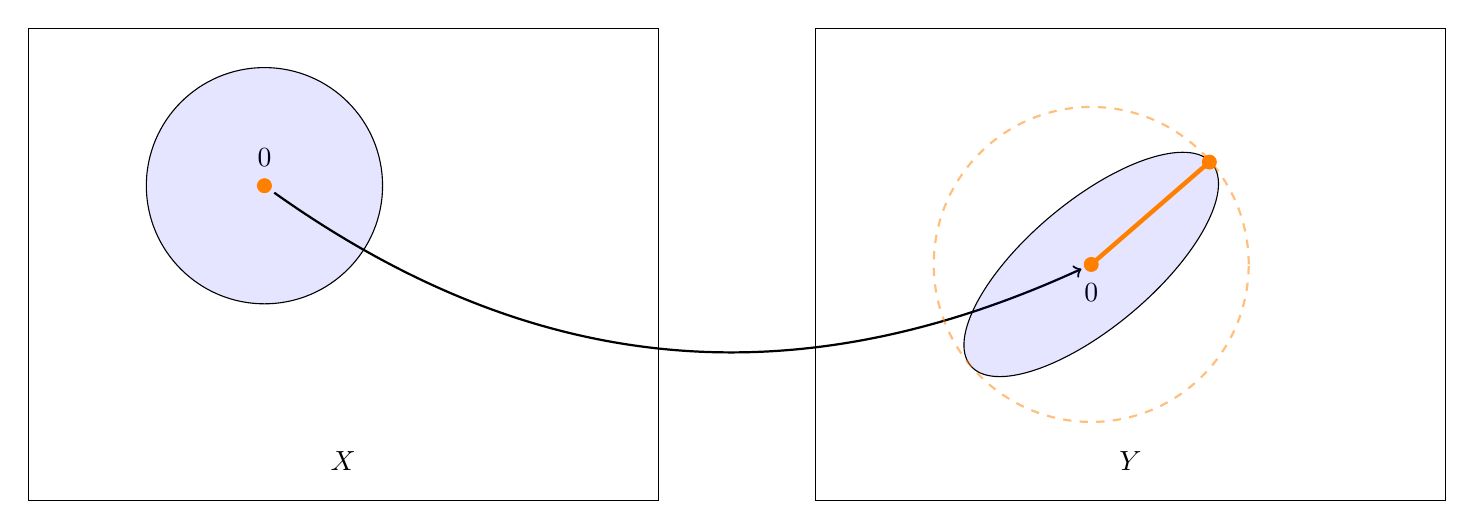
\begin{tikzpicture}
    \draw (0,0) rectangle (8,6);\node at (4,0.5) {$X$};
    \node[label=$0$]  (p) at (3,4) {};
    \draw[fill =blue,fill opacity=0.1] (p)  circle (1.5cm);
    \draw [orange] plot [only marks, mark size=2.5, mark=*] coordinates {(3,4)};

    \draw (10,0) rectangle (18,6);\node at (14,0.5) {$Y$};
    \node[label=below:$0$]  (p') at (13.5,3.0) {};
    
    \draw[thick,->] (p) edge[bend right] (p');
    \draw[fill =blue,fill opacity=0.1,rotate=310] (p') ellipse (0.8cm and 2cm);

    \draw[ultra thick, orange] (13.5,3.0) -- (15.0,4.3);
    \draw [orange] plot [only marks, mark size=2.5, mark=*] coordinates {(13.5,3.0)};
    \draw [orange] plot [only marks, mark size=2.5, mark=*] coordinates {(15.0,4.3)};

    \draw[orange, dashed, opacity=0.5, thick] (p') circle (2cm);
\end{tikzpicture}
\end{center}

\vspace*{7mm}

Заведем еще парОчку (пять) способов посчитать норму. 
\begin{theorem}
    \begin{align}
        \sup\limits_{\norm{x}_X \leqslant 1} \norm{\A x}_Y &= \\
        &= \sup\limits_{\norm{x}_X < 1} \norm{\A x}_Y \\
        &= \sup\limits_{\norm{x}_X = 1} \norm{\A x}_Y \\
        &= \sup\limits_{x \neq 0} \frac{\norm{\A x}_Y}{\norm{x}_X} \\
        &= \inf{\{ C \in \R : \forall x \in X \quad \norm{\A x}_Y \leqslant C \norm{x}_X \}}
    \end{align}
\end{theorem}
\newcommand{\tikzmark}[1]{\tikz[overlay,remember picture] \node (#1) {};}
\newcommand{\DrawBox}[1]{%
  \begin{tikzpicture}[overlay,remember picture]
    \draw[->,shorten >=5pt,shorten <=5pt,out=50,in=100,distance=0.7cm,#1, thick] ($(MarkA.north)+(.4em,.4em)$) to (MarkB.north);
    \draw[overlay,red,thick,dashed] ($(MarkA)!.5!(MarkABot)+(.4em,.2em)$) ellipse (0.6cm and 0.8cm);
  \end{tikzpicture}
}
\begin{proof} \quad 

    Очевидно, что $(1) \geqslant (2)$ и $(1) \geqslant (3)$ так как в $N_1$ множество больше.

    $(3) = (4)$:
    \begin{gather*}
        \frac{\norm{\A x}_Y}{\norm{x}_X} = \frac{1\tikzmark{MarkA}}{\tikzmark{MarkABot}\norm{x}_X} \cdot \norm{\A \tikzmark{MarkB} x}_Y\DrawBox{red} =
        \norm{\A \bigg( \underbrace{\colorboxed{red}{\frac{x}{\norm{x}_X}}}_{\text{единичн. век.}}\bigg)} \leqslant (3)
    \end{gather*}
    Дробь под оператор занесли по линейности. Так как под операторов получили единичный вектор, то это подмножество $(3)$. 
    Рассматривая в $(4)$ только иксы подходящие в третьем получаем обратное неравенство. Значит выполняется равенство.

    $(4) = (5)$:

    $(4) = $ наименьшая верхняя граница для $\frac{\norm{\A x}_Y}{\norm{x}_X}$. Переформулируем и распишем:
    \begin{gather*}
        (4) = \min \{ C : \frac{\norm{\A x}_Y}{\norm{x}_X} \leqslant C \} = \min \{ C : \norm{\A x}_Y \leqslant C \norm{x}_X\}
    \end{gather*}
    Получили $(5)$, но по $x \neq 0$, так как это было сказано в $(4)$, но, для $x = 0$ неравенство в принципе всегда выполняется, так что все хорошо.

    $(3) \geqslant (1)$:

    \begin{align*}
        \norm{\A x}_Y &= \norm{\A \left( \frac{x}{\norm{x}_X} \cdot \norm{x}_X \right)} \\
        &= \norm{x}_X \cdot \norm{\A \left( \frac{x}{\norm{x}_X} \right)} \text{ по линейности} \\
        &\leqslant \oast
    \end{align*}
    $\oast \leqslant \norm{x}_X \cdot (3)$, так как в $(3)$ тоже единичный вектор, но там стоит значек супремума. А это в свою очередь 
    не превосходит $(3)$, так как норма $x$ не превосходит единицы.

    $(2) \geqslant (1)$:

    Берем $x$ по норме не превосходящие 1. Тогда:
    \begin{gather*}
        \norm{(1 - \varepsilon)x}_X \leqslant 1 - \varepsilon < 1 \Longrightarrow \stackbelow{\underbrace{\sup\limits_{\norm{x}_X \leqslant 1} \norm{\A ((1-\varepsilon)x)}_Y}}{\oast} \leqslant (2)
    \end{gather*}
    Вынесем $(1 - \varepsilon)$ совсем наружу, потому что это вообще положительная константа и мы так можем. Тогда получим:
    \begin{gather*}
        \oast = (1 - \varepsilon) \sup\limits_{\norm{x}_X \leqslant 1} \norm{\A x}_Y = (1 - \varepsilon) \cdot (1) \\
        \Longrightarrow (1 - \varepsilon) \cdot (1) \leqslant (2) \quad \forall \varepsilon > 0
    \end{gather*}
    Тогда устремляем $\varepsilon$ к нулю и получим нужное неравенство.
\end{proof}
\textbf{Следствия: }
\begin{enumerate}
    \item $\norm{\A x}_Y \leqslant \norm{\A} \cdot \norm{x}_X$
    \item $\norm{\A \B} \leqslant \norm{\A} \cdot \norm{\B}$
\end{enumerate}
\begin{proof} \quad 

    \begin{enumerate}
        \item \begin{gather*}
            \norm{\A} = \sup\limits_{x \neq 0} \frac{\norm{\A x}_Y}{\norm{x}_X} \Longrightarrow \norm{\A x}_Y \leqslant \norm{\A} \cdot \norm{x}_X \text{ при } x \neq 0
        \end{gather*}
        \item Распишем норму $\A \B$:
        \begin{gather*}
            \norm{\A \B} = \sup\limits_{x \neq 0} \frac{\norm{\A \B x}_Z}{\norm{x}_X} \leqslant \oast
        \end{gather*}
        По определению: $\B : X \longrightarrow Y, \A : Y \longrightarrow Z$. Тогда:
        \begin{gather*}
            \norm{\A \B x}_Z = \norm{\A} \cdot \norm{\B x}_Y \leqslant \norm{\A} \cdot \norm{\B} \cdot \norm{x}_X
        \end{gather*}
        Подставим оценОчку:
        \begin{gather*}
            \oast \leqslant \sup\limits_{x \neq 0} \frac{\norm{\A} \cdot \norm{\B} \cdot \cancel{\norm{x}_X}}{\cancel{\norm{x}_X}} = \norm{\A} \cdot \norm{\B}
        \end{gather*}
    \end{enumerate}
\end{proof}
\begin{theorem}
    $\A : X \longrightarrow Y$ линейный оператор. Тогда равносильны:
    \begin{enumerate}
        \item $\A$ -- ограниченный оператор 
        \item $\A$ непрерывен в нуле 
        \item $\A$ непрерывен везде
        \item $\A$ равномерно непрерывен 
    \end{enumerate}
\end{theorem}
\begin{proof}
    $4. \Longrightarrow 3. \Longrightarrow 2.$ очевидно 

    $1. \Longrightarrow 4$:
    
    \begin{gather*}
        \norm{\A x - \A y} = \norm{\A (x-y)} \leqslant \norm{\A} \cdot \norm{x - y} < \varepsilon \text{ если } \norm{x - y} < \delta
    \end{gather*}
    Тогда понятно, какую дельту нужно взять. Просто возьмем $\delta := \frac{\varepsilon}{\norm{\A}}$. Тогда если у нас $x$ от $y$ 
    отличается меньше, чем на $\delta$, то $\A x$ будет отличаться от $\A y$ меньше чем на $\varepsilon$. Вот и равномерная непрерывность.

    $2. \longrightarrow 1.$:

    Берем $\varepsilon = 1$ и $\delta > 0$ по нему. Тогда:
    \begin{gather*}
        \forall x \in X : \norm{x} < \delta \Longrightarrow \norm{\A x} < 1
    \end{gather*}
    Если $\norm{y} < 1$, то:
  \begin{gather*}
    \norm{\delta y} < \delta \Longrightarrow \stackbelow{\norm{\underbrace{\A (\delta y)}}}{\delta \norm{\A y}} < 1 \\
    \Longrightarrow \norm{\A y} < \frac{1}{\delta} \Longrightarrow \norm{\A} = \sup\limits_{\norm{y} < 1} \norm{\A y} \leqslant \frac{1}{\delta}
  \end{gather*}
  А значит оператор $\A$ ограничен.
\end{proof}